\chapter{Protocole de communication informatique}
Nous considérons maintenant un système de communication informatique mis en place entre un client et deux serveurs, un serveur principal et un autre de secours utilisé quand le premier tombe en panne. Le but du système est de permettre au client de pouvoir envoyer deux types de messages : $m_1$ et $m_2$  l'aide de l'un des deux serveur.

Nous avons alors choisi de représenter le modèle du procédé de ce système par l'automate suivant :
\begin{figure}[!ht]
\begin{minipage}{0.5\textwidth}
\centering
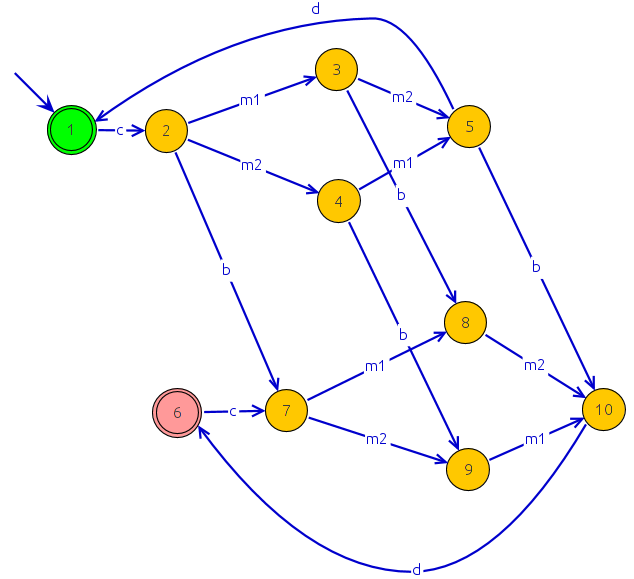
\includegraphics[width = \textwidth]{./III/images/P.png}
\caption{Modèle de procédé}
\end{minipage}
\begin{minipage}{0.5\textwidth}
Avec : \begin{itemize}[label = \textbullet]
\item $\Sigma_P = \left\lbrace m_1, m_2, b, c, d \right\rbrace$
\item $\Sigma_O =  \left\lbrace m_1, m_2, b, c, d \right\rbrace$
\end{itemize}
\end{minipage}
\end{figure}
Soit avec la particularité suivante : une fois que le serveur est tombé en panne, celui ci nécessite une dépannage manuel et donc l'automate serait ré-intialisé. 

Les spécifications de notre système sont que chaque l'émission des messages vers le serveur doivent respectés l'ordre $m_1 \rightarrow m_2$, nous obtenons l'automate 
\begin{center}
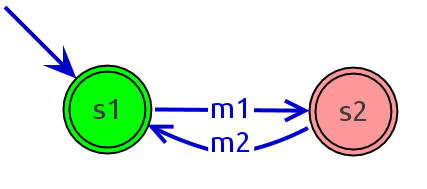
\includegraphics[width = .5\textwidth]{./III/images/S.png}
\captionof{figure}{Modèle des spécifications}
\end{center}
Nous pouvons maintenant calculé avec un produit parallèle et DESUMA la commande supervisé que nous allons appliquer. Nous seront aptes par la suite à déterminer les propriétés de notre commande. L'automate est :\begin{figure}[!ht]
\begin{minipage}{.5\textwidth}
\centering
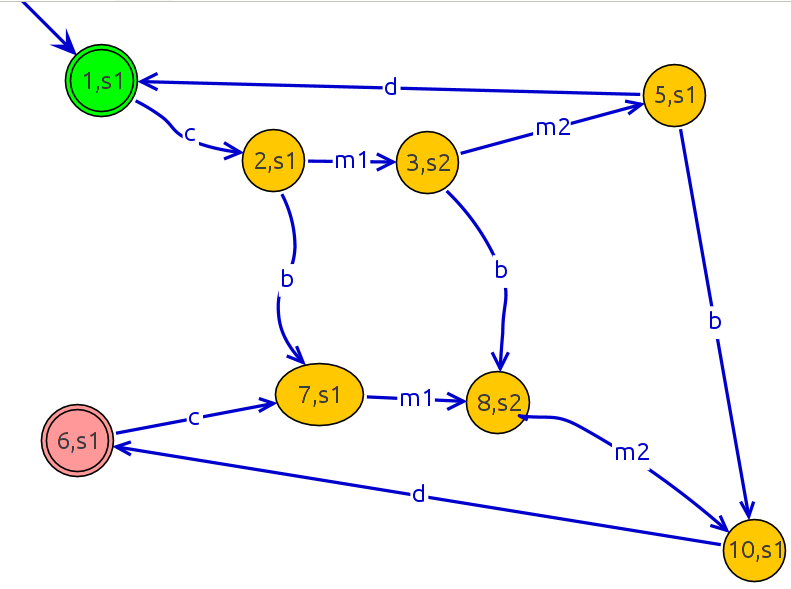
\includegraphics[width=\textwidth]{./III/images/P_S.png}
\caption{Modèle de commande supervisée}
\end{minipage} \hfill
\begin{minipage}{.5\textwidth}
\centering
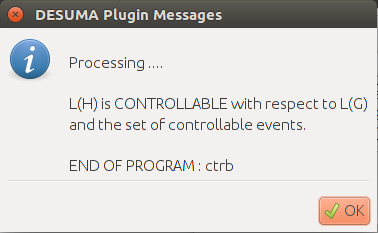
\includegraphics[width=\textwidth]{./III/images/P_S_ctrbl.png}
\caption{Message DESUMA sur la contrôlabilité}
\end{minipage}
\end{figure}

L'algorithme de vérification de DESUMA n'a pas trouvé de séquence d'évènements non contrôlable ne respectant pas $S$, notre commande est donc contrôlable. Les états marqués $(1,s1)$ et $(6,s1)$ sont accessibles par n'importe quel état, la commande est donc non-blocante.